%%%%%%%%%%%%%%%%%%%%%%%%%%%%%%%%%%%%%%%%%%%%%%%%%%%%%%%%%%%%%%%%%%%%%%%%
% Chapter: MPOPF Modelling Tradeoffs - Linear vs Nonlinear
% Context: Formulation choices before decomposition  
%%%%%%%%%%%%%%%%%%%%%%%%%%%%%%%%%%%%%%%%%%%%%%%%%%%%%%%%%%%%%%%%%%%%%%%%
\clearpage
\section{MPOPF Modelling Tradeoffs: Linear vs Nonlinear Formulations}

%%%%%%%%%%%%%%%%%%%%%%%%%%%%%%%%%%%%%%%%%%%%%%%%%%%%%%%%%%%%%%%%%%%%%%%%
\subsection{Introduction}
%%%%%%%%%%%%%%%%%%%%%%%%%%%%%%%%%%%%%%%%%%%%%%%%%%%%%%%%%%%%%%%%%%%%%%%%

Before applying spatial or temporal decomposition to multi-period optimal power flow (MPOPF) problems, a critical decision must be made: \textbf{which power flow formulation to use?} This chapter compares two approaches:

\begin{enumerate}
    \item \textbf{Nonlinear Branch Flow Model (BFM-NL)} \cite{Farivar1}: Accurate non-convex programming, computationally expensive
    \item \textbf{LinDistFlow} \cite{Gan}: Fast linear programming with approximation errors
\end{enumerate}

\textbf{Key Insight:} The formulation choice shapes any decomposition algorithm built upon it. Even if decomposition converges correctly, a flawed base formulation propagates errors.

This chapter establishes theoretical foundations (problem definition, formulations, performance metrics), then presents empirical results demonstrating the tradeoffs for systems of varying scales and grid-edge device (GED) penetrations.

%%%%%%%%%%%%%%%%%%%%%%%%%%%%%%%%%%%%%%%%%%%%%%%%%%%%%%%%%%%%%%%%%%%%%%%%
\subsection{MPOPF Problem Definition}
%%%%%%%%%%%%%%%%%%%%%%%%%%%%%%%%%%%%%%%%%%%%%%%%%%%%%%%%%%%%%%%%%%%%%%%%

\paragraph{System Model:} Radial distribution network as a tree with buses $\mathcal{N}$, lines $\mathcal{L}$, time horizon $\tau = \{1, \ldots, T\}$, load buses $\mathcal{N_L}$, PV buses $\mathcal{D} \subseteq \mathcal{N_L}$, battery buses $\mathcal{B} \subseteq \mathcal{N_L}$.

\paragraph{Key Variables:} $v_j^t = (V_j^t)^2$ (squared voltage), $l_{ij}^t = (I_{ij}^t)^2$ (squared current), $P_{ij}^t, Q_{ij}^t$ (line flows), $p^t_{D_j}, q^t_{D_j}$ (PV output), $P_{c_j}^t, P_{d_j}^t, q_{B_j}^t$ (battery power), $B_j^t$ (battery energy), $P^t_{Subs}$ (substation power), $C^t$ (electricity cost).

\paragraph{Objective Function:} Minimize total substation cost plus penalty for simultaneous charge-discharge \cite{Nazir2021Sep}:
\begin{align}
    \min \sum_{t=1}^{T} \left\{ C^t P^t_{Subs} \Delta t + \alpha \sum_{j \in \mathcal{B}} \left[ (1-\eta_c)P^t_{c_j} + \left( \tfrac{1}{\eta_d} - 1 \right) P^t_{d_j} \right] \right\}
    \label{eq:mpopf-obj}
\end{align}

%%%%%%%%%%%%%%%%%%%%%%%%%%%%%%%%%%%%%%%%%%%%%%%%%%%%%%%%%%%%%%%%%%%%%%%%
\subsection{Formulation Comparison}
%%%%%%%%%%%%%%%%%%%%%%%%%%%%%%%%%%%%%%%%%%%%%%%%%%%%%%%%%%%%%%%%%%%%%%%%

\Cref{table:mpopf-formulation-comparison} contrasts the two formulations.

\begin{table}[h]
    \centering
    \caption{BFM-NL vs LinDistFlow formulation comparison}
    \label{table:mpopf-formulation-comparison}
    \small
    \begin{tabular}{|l|l|l|}
    \hline
    \textbf{Constraint} & \textbf{BFM-NL} & \textbf{LinDistFlow} \\ \hline
    Real power balance & $\sum_k P_{jk}^t - (P_{ij}^t - r_{ij}l_{ij}^t) = p_j^t$ & $\sum_k P_{jk}^t - P_{ij}^t = p_j^t$ \\ \hline
    Reactive power balance & $\sum_k Q_{jk}^t - (Q_{ij}^t - x_{ij}l_{ij}^t) = q_j^t$ & $\sum_k Q_{jk}^t - Q_{ij}^t = q_j^t$ \\ \hline
    Voltage drop (KVL) & $v_j^t = v_i^t - 2(r_{ij}P_{ij}^t + x_{ij}Q_{ij}^t) + (r_{ij}^2+x_{ij}^2)l_{ij}^t$ & $v_j^t = v_i^t - 2(r_{ij}P_{ij}^t + x_{ij}Q_{ij}^t)$ \\ \hline
    Power-current relation & $(P_{ij}^t)^2 + (Q_{ij}^t)^2 = l_{ij}^t v_i^t$ & Not modeled \\ \hline
    Battery inverter & $(P_{B_j}^t)^2 + (q_{B_j}^t)^2 \leq S_{B_{R,j}}^2$ & Hexagonal approx. \cite{Ahmadi2014Oct} \\ \hline
    \end{tabular}
\end{table}

\textbf{Key Differences:} BFM-NL includes loss terms $(r_{ij}l_{ij}^t, x_{ij}l_{ij}^t)$ and quadratic constraints; LinDistFlow drops these for linearity, introducing approximation errors.

\textbf{Common Constraints:} Voltage limits $v_j^t \in [V_{min}^2, V_{max}^2]$, battery dynamics $B_j^t = B_j^{t-1} + \Delta t(\eta_c P_{c_j}^t - \eta_d^{-1} P_{d_j}^t)$, power limits, SOC bounds.

%%%%%%%%%%%%%%%%%%%%%%%%%%%%%%%%%%%%%%%%%%%%%%%%%%%%%%%%%%%%%%%%%%%%%%%%
\subsection{Performance Metrics}
%%%%%%%%%%%%%%%%%%%%%%%%%%%%%%%%%%%%%%%%%%%%%%%%%%%%%%%%%%%%%%%%%%%%%%%%

\paragraph{Optimality:} Gap between objective values:
\begin{equation}
    \text{Optimality Gap (\%)} = \frac{\text{Cost}_{\text{LinDistFlow}} - \text{Cost}_{\text{BFM-NL}}}{\text{Cost}_{\text{BFM-NL}}} \times 100
\end{equation}

\paragraph{Feasibility:} Discrepancies when control set-points are validated in OpenDSS (AC power flow):
\begin{align}
    \Delta V = \max_{j,t} |V^t_{j,\text{OpenDSS}} - V^t_{j,\text{model}}|, \quad
    \Delta P_{Subs} = \max_{t} |P^t_{Subs,\text{OpenDSS}} - P^t_{Subs,\text{model}}|
\end{align}

\paragraph{Computational Efficiency:} Wall-clock solve time (seconds) using Ipopt \cite{ipopt-solver-Wachter2006Mar} via JuMP \cite{Lubin2023}.

%%%%%%%%%%%%%%%%%%%%%%%%%%%%%%%%%%%%%%%%%%%%%%%%%%%%%%%%%%%%%%%%%%%%%%%%
\subsection{Empirical Evaluation}
%%%%%%%%%%%%%%%%%%%%%%%%%%%%%%%%%%%%%%%%%%%%%%%%%%%%%%%%%%%%%%%%%%%%%%%%

\subsubsection{Test Systems}

Three systems with increasing size and GED penetration (PV\%/BESS\%):
\begin{itemize}
    \item \textbf{ADS10}: 10-bus, 25\%/25\%, 33\% sizing (\Cref{fig:mpopf-ads10})
    \item \textbf{IEEE123A}: 128-bus, 20\%/30\%, 33\% sizing (\Cref{fig:mpopf-ieee123})
    \item \textbf{IEEE123B}: 128-bus, 30\%/50\%, 100\% sizing
\end{itemize}

\begin{figure}[h]
    \centering
    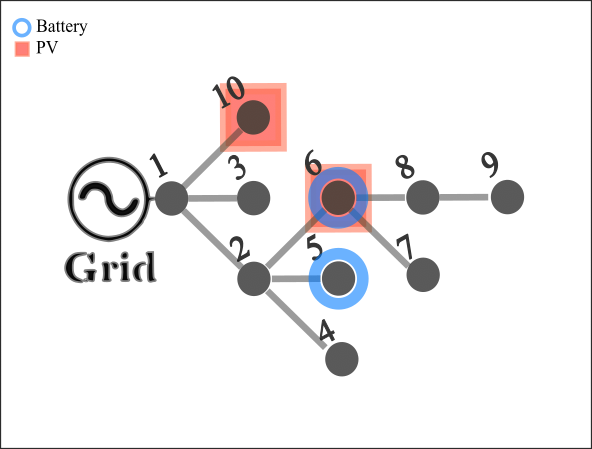
\includegraphics[width=0.55\linewidth]{figures/ads10-pv25-batt25.png}
    \caption{ADS10: 10-bus system}
    \label{fig:mpopf-ads10}
\end{figure}

\begin{figure}[h]
    \centering
    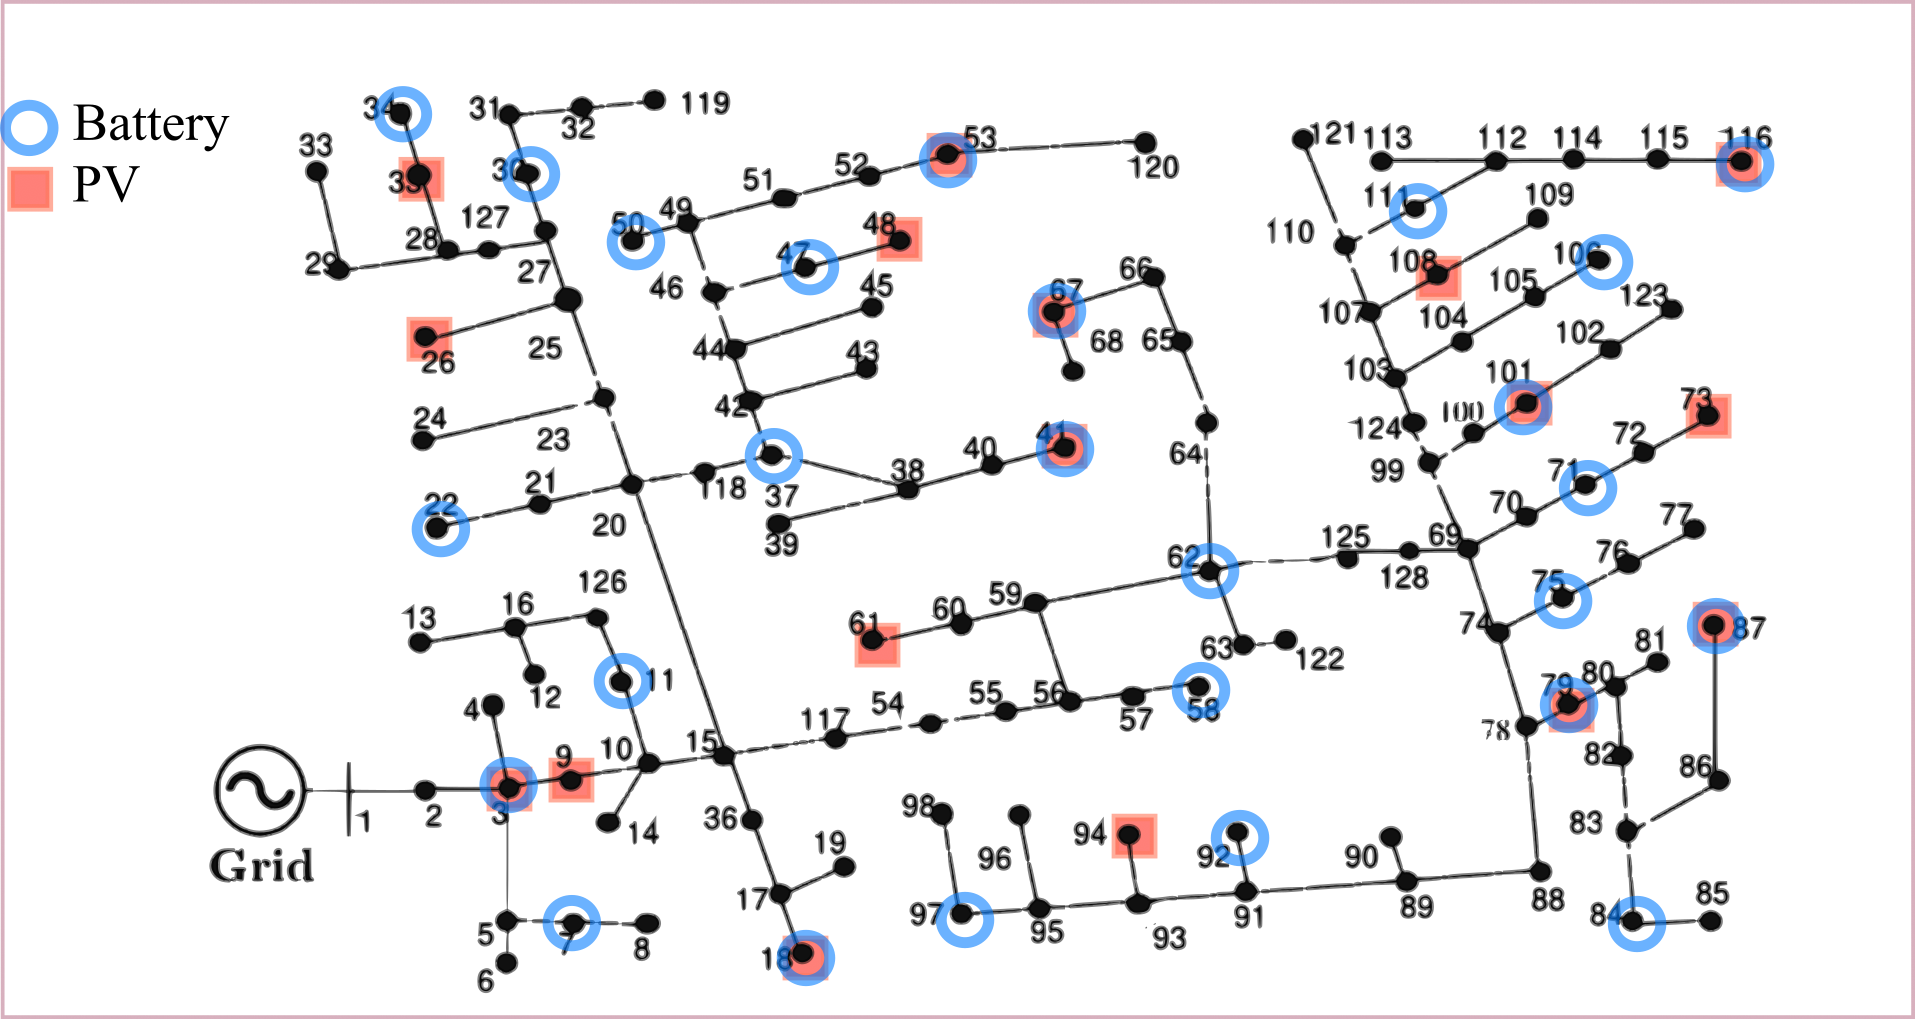
\includegraphics[width=0.8\linewidth]{figures/ieee123-pv20-batt30.png}
    \caption{IEEE-123: 128-bus system}
    \label{fig:mpopf-ieee123}
\end{figure}

All systems use 24-hour forecasts (\Cref{fig:mpopf-input}) with bilevel pricing. Parameters: $T=24$ h, $\Delta t=1$ h, $V_{min/max}=0.95/1.05$ pu, $\eta_c=\eta_d=0.95$, $soc_{min/max}=0.30/0.95$, 4-hour battery storage.

\begin{figure}[h]
    \centering
    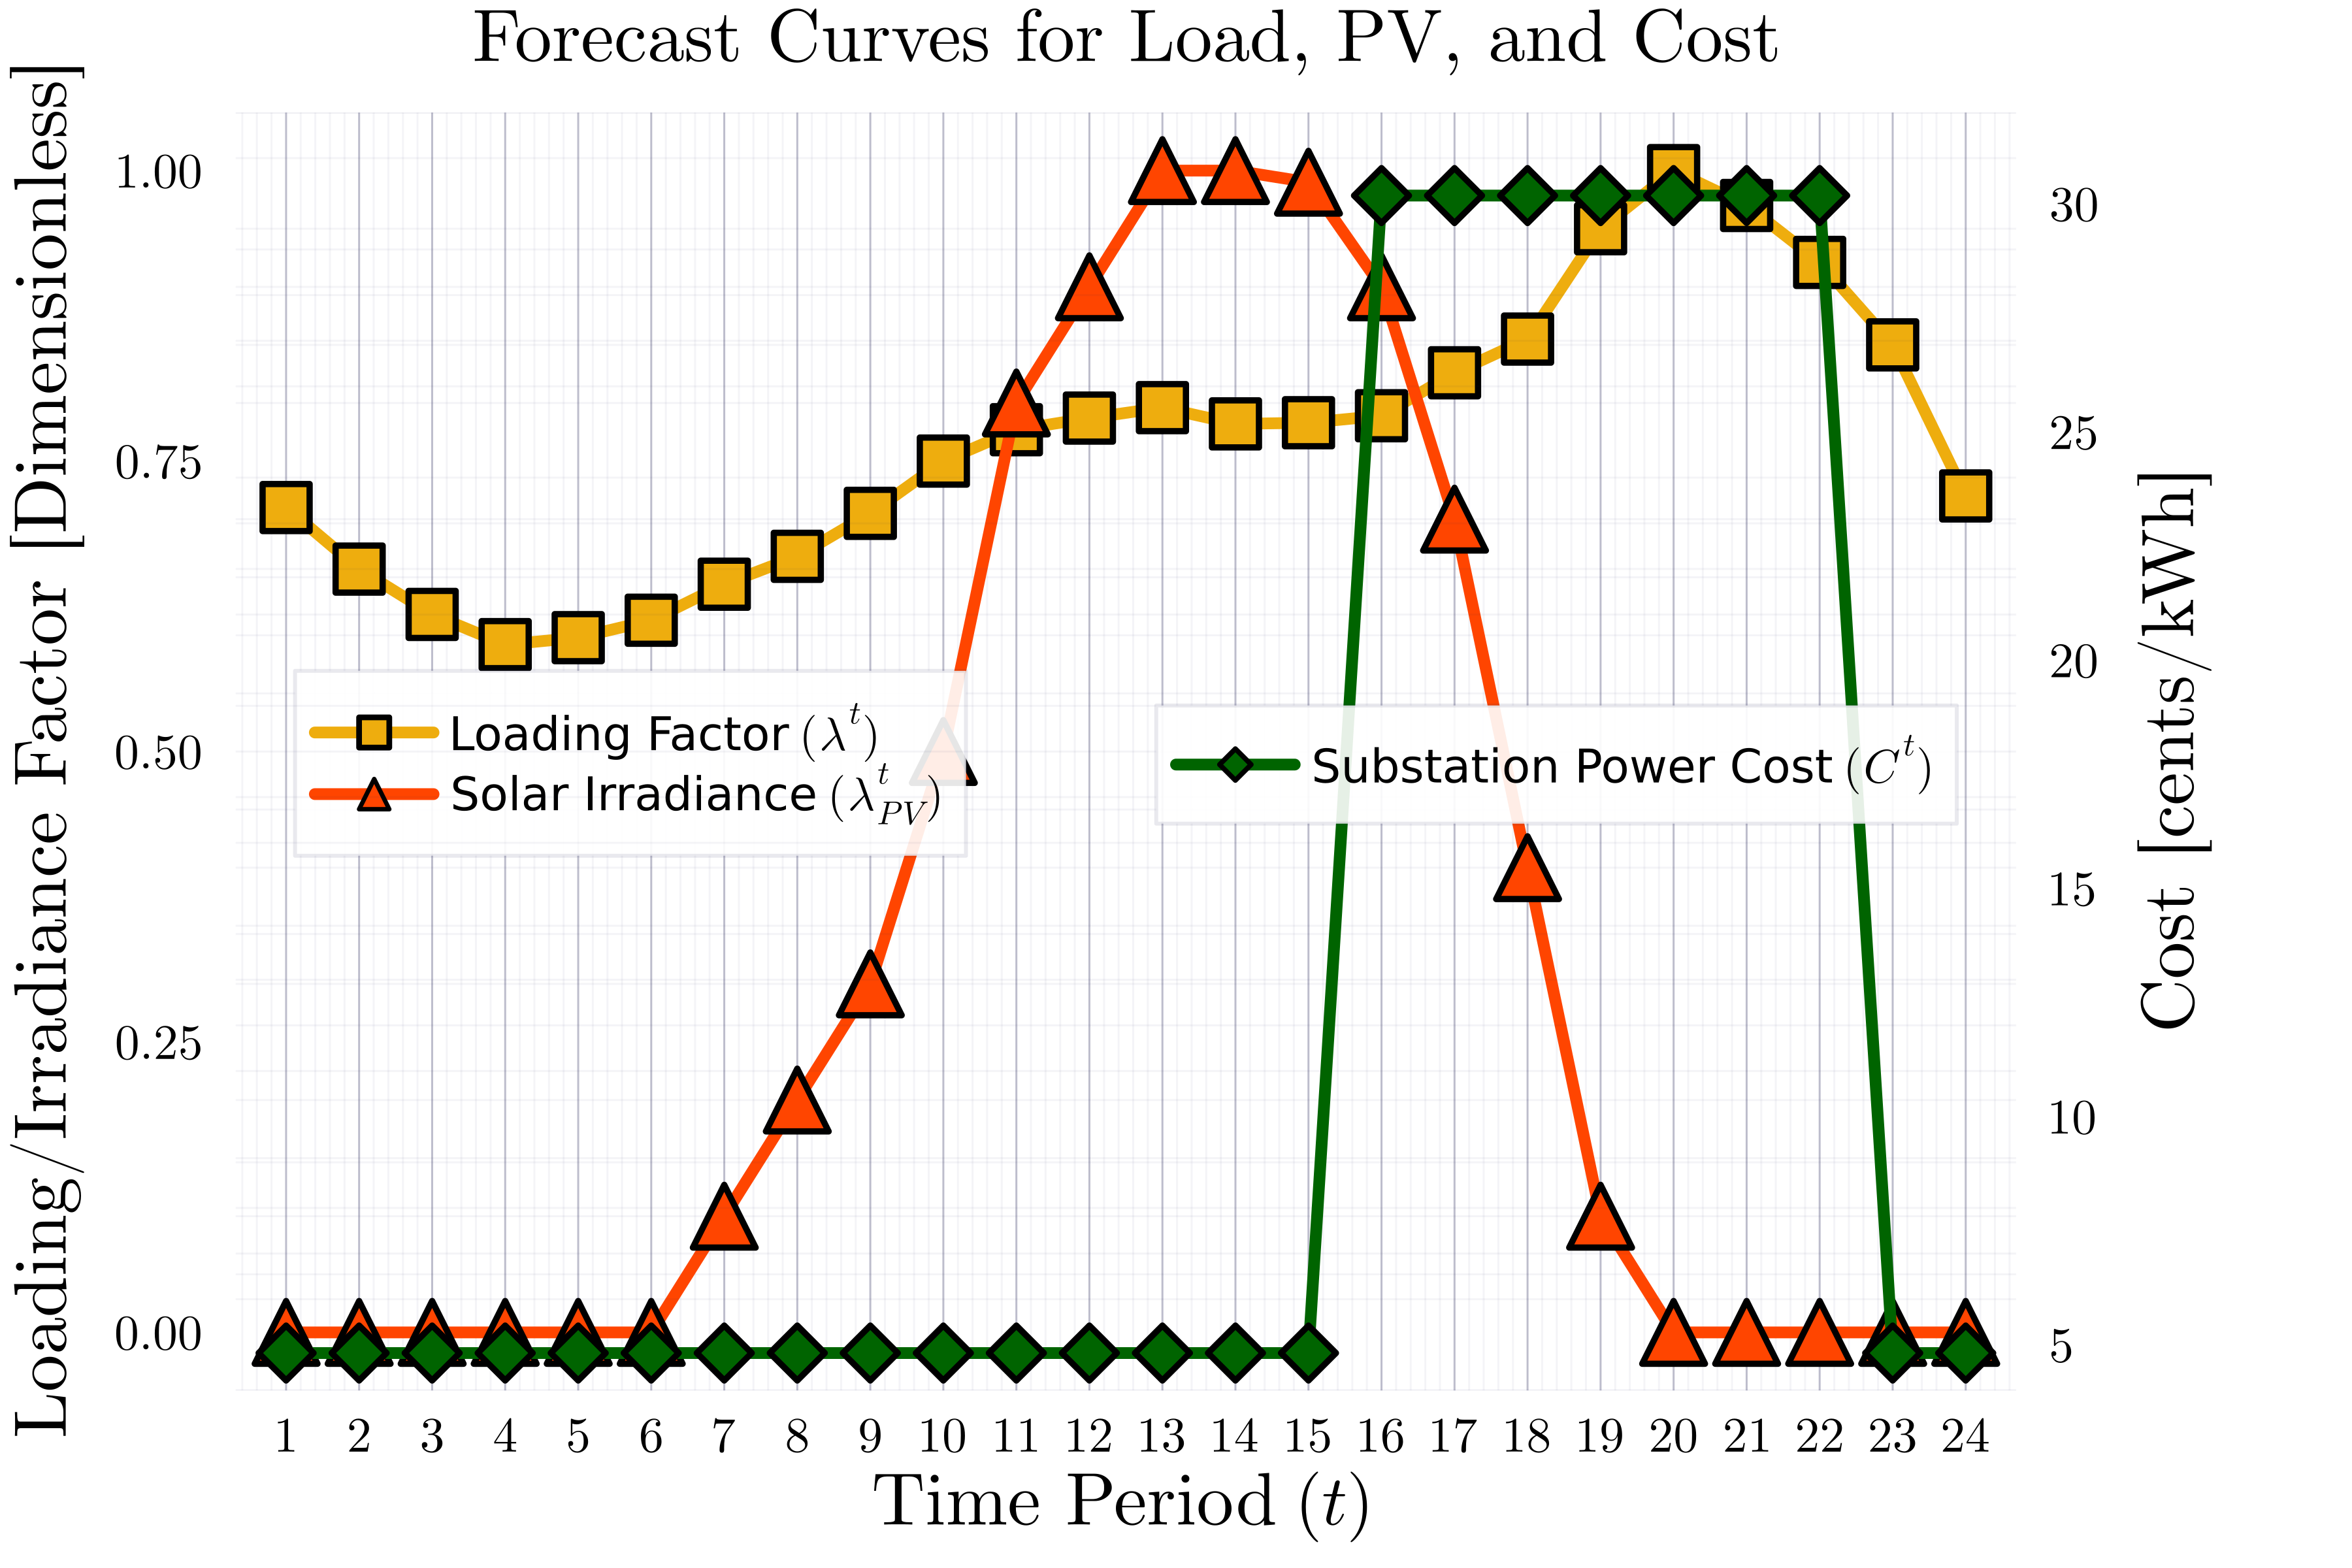
\includegraphics[height=0.2\textheight]{figures/T24-inputCurves/Horizon_24_InputForecastCurves_bilevelCosts.png}
    \caption{24-hour forecasts: load, irradiance, cost}
    \label{fig:mpopf-input}
\end{figure}

\subsubsection{Workflow}

Models built in JuMP, solved with Ipopt (cold start). Control set-points validated in OpenDSS via OpenDSSDirect.jl \cite{OpenDSSDirect-jl}. Code: \cite{MPOPFRepo}.

\textbf{Note:} LinDistFlow$^{\mathbb{O}}$ denotes LinDistFlow controls evaluated in OpenDSS (to account for actual losses).

\subsubsection{Results}

\Cref{table:mpopf-results-summary} summarizes key findings across all three systems.

\begin{table}[h]
    \centering
    \caption{Performance summary: BFM-NL vs LinDistFlow}
    \label{table:mpopf-results-summary}
    \small
    \begin{tabular}{|l|c|c|c|c|c|c|}
    \hline
    \multirow{2}{*}{\textbf{Metric}} & \multicolumn{2}{c|}{\textbf{ADS10}} & \multicolumn{2}{c|}{\textbf{IEEE123A}} & \multicolumn{2}{c|}{\textbf{IEEE123B}} \\ \cline{2-7}
    & BFM-NL & LinDF$^{\mathbb{O}}$ & BFM-NL & LinDF$^{\mathbb{O}}$ & BFM-NL & LinDF$^{\mathbb{O}}$ \\ \hline
    Cost (\$) & 204.27 & 204.28 & 2787.44 & 2798.4 & 1973.83 & 1987.78 \\ \hline
    Optimality gap (\%) & \multicolumn{2}{c|}{0.005} & \multicolumn{2}{c|}{0.39} & \multicolumn{2}{c|}{0.71} \\ \hline
    Solve time (s) & 2.64 & 0.77 & 17.44 & 0.85 & 23.75 & 1.66 \\ \hline
    Speedup & \multicolumn{2}{c|}{3.4×} & \multicolumn{2}{c|}{20.5×} & \multicolumn{2}{c|}{14.3×} \\ \hline
    $\Delta V$ (pu) & 0.00001 & 0.00001 & 0.00007 & 0.00206 & 0.00006 & 0.00160 \\ \hline
    $\Delta P_{Subs}$ (kW) & 0.00001 & 0.02 & 0.43 & 32.36 & 0.22 & 23.34 \\ \hline
    \end{tabular}
\end{table}

%%%%%%%%%%%%%%%%%%%%%%%%%%%%%%%%%%%%%%%%%%%%%%%%%%%%%%%%%%%%%%%%%%%%%%%%
\subsection{Discussion}
%%%%%%%%%%%%%%%%%%%%%%%%%%%%%%%%%%%%%%%%%%%%%%%%%%%%%%%%%%%%%%%%%%%%%%%%

\paragraph{Optimality Gap:} Grows from 0.005\% (ADS10) to 0.71\% (IEEE123B) due to: (1) larger line losses not captured by LinDistFlow, (2) higher battery penetration amplifying hexagonal approximation error. \textbf{Implication:} For decomposition algorithms, LinDistFlow provides acceptable cost approximations for small-moderate systems but degrades with scale.

\paragraph{Computational Speedup:} LinDistFlow achieves 3×–20× faster solve times by eliminating nonlinear constraints. \textbf{Implication:} Useful for rapid initialization or warm-starting BFM-NL-based decomposition.

\paragraph{Reactive Power Mismanagement:} LinDistFlow allocates 10×–18× less reactive power to distributed inverters compared to BFM-NL (e.g., IEEE123A: 195 vs 1972 kVARh for PVs), concentrating support at the substation. This stems from omitting the $l_{ij}^t x_{ij}$ term that couples reactive flow to losses. \textbf{Implication:} Under-utilizes grid support capability; risky for voltage regulation objectives.

\paragraph{Substation Power Underprediction:} LinDistFlow underestimates hourly substation power by up to 32 kW (2–5\%), creating risks: equipment overloads, reserve margin violations, economic errors. \textbf{Implication:} Decomposition algorithms using LinDistFlow will systematically underpredict system-level quantities.

\paragraph{Recommended Strategy:} \textbf{Hybrid approach} for decomposition: (1) Initialize with LinDistFlow for speed, (2) Refine with BFM-NL for accuracy, (3) Validate with OpenDSS before deployment. This balances computational tractability with solution quality.

%%%%%%%%%%%%%%%%%%%%%%%%%%%%%%%%%%%%%%%%%%%%%%%%%%%%%%%%%%%%%%%%%%%%%%%%
\subsection{Conclusions}
%%%%%%%%%%%%%%%%%%%%%%%%%%%%%%%%%%%%%%%%%%%%%%%%%%%%%%%%%%%%%%%%%%%%%%%%

The formulation choice (BFM-NL vs LinDistFlow) fundamentally determines the behavior of any spatial or temporal decomposition algorithm. Key takeaways:

\begin{itemize}
    \item \textbf{Optimality:} LinDistFlow introduces 0.4–0.7\% gap for moderate-large systems
    \item \textbf{Reactive Power:} LinDistFlow systematically misallocates reactive resources
    \item \textbf{Feasibility:} Substation power errors up to 5\% create operational risks
    \item \textbf{Speed:} 10–20× computational advantage enables rapid scenario analysis
\end{itemize}

For the spatial (ENApp) and temporal (ADMM) decomposition algorithms in subsequent chapters, this analysis informs whether to use BFM-NL (accurate but slow), LinDistFlow (fast but approximate), or a hybrid strategy depending on system scale and accuracy requirements.

\textbf{The aim of this thesis is to develop decomposition algorithms based on the accurate BFM-NL formulation to ensure high-fidelity solutions for large-scale MPOPF problems.}

But it is also important to recognize the potential role of LinDistFlow in initialization or warm-starting to accelerate convergence without sacrificing final solution quality.
